\documentclass[twoside]{book}

% Packages required by doxygen
\usepackage{fixltx2e}
\usepackage{calc}
\usepackage{doxygen}
\usepackage[export]{adjustbox} % also loads graphicx
\usepackage{graphicx}
\usepackage[utf8]{inputenc}
\usepackage{makeidx}
\usepackage{multicol}
\usepackage{multirow}
\PassOptionsToPackage{warn}{textcomp}
\usepackage{textcomp}
\usepackage[nointegrals]{wasysym}
\usepackage[table]{xcolor}

% Font selection
\usepackage[T1]{fontenc}
\usepackage[scaled=.90]{helvet}
\usepackage{courier}
\usepackage{amssymb}
\usepackage{sectsty}
\renewcommand{\familydefault}{\sfdefault}
\allsectionsfont{%
  \fontseries{bc}\selectfont%
  \color{darkgray}%
}
\renewcommand{\DoxyLabelFont}{%
  \fontseries{bc}\selectfont%
  \color{darkgray}%
}
\newcommand{\+}{\discretionary{\mbox{\scriptsize$\hookleftarrow$}}{}{}}

% Page & text layout
\usepackage{geometry}
\geometry{%
  a4paper,%
  top=2.5cm,%
  bottom=2.5cm,%
  left=2.5cm,%
  right=2.5cm%
}
\tolerance=750
\hfuzz=15pt
\hbadness=750
\setlength{\emergencystretch}{15pt}
\setlength{\parindent}{0cm}
\setlength{\parskip}{3ex plus 2ex minus 2ex}
\makeatletter
\renewcommand{\paragraph}{%
  \@startsection{paragraph}{4}{0ex}{-1.0ex}{1.0ex}{%
    \normalfont\normalsize\bfseries\SS@parafont%
  }%
}
\renewcommand{\subparagraph}{%
  \@startsection{subparagraph}{5}{0ex}{-1.0ex}{1.0ex}{%
    \normalfont\normalsize\bfseries\SS@subparafont%
  }%
}
\makeatother

% Headers & footers
\usepackage{fancyhdr}
\pagestyle{fancyplain}
\fancyhead[LE]{\fancyplain{}{\bfseries\thepage}}
\fancyhead[CE]{\fancyplain{}{}}
\fancyhead[RE]{\fancyplain{}{\bfseries\leftmark}}
\fancyhead[LO]{\fancyplain{}{\bfseries\rightmark}}
\fancyhead[CO]{\fancyplain{}{}}
\fancyhead[RO]{\fancyplain{}{\bfseries\thepage}}
\fancyfoot[LE]{\fancyplain{}{}}
\fancyfoot[CE]{\fancyplain{}{}}
\fancyfoot[RE]{\fancyplain{}{\bfseries\scriptsize Generated by Doxygen }}
\fancyfoot[LO]{\fancyplain{}{\bfseries\scriptsize Generated by Doxygen }}
\fancyfoot[CO]{\fancyplain{}{}}
\fancyfoot[RO]{\fancyplain{}{}}
\renewcommand{\footrulewidth}{0.4pt}
\renewcommand{\chaptermark}[1]{%
  \markboth{#1}{}%
}
\renewcommand{\sectionmark}[1]{%
  \markright{\thesection\ #1}%
}

% Indices & bibliography
\usepackage{natbib}
\usepackage[titles]{tocloft}
\setcounter{tocdepth}{3}
\setcounter{secnumdepth}{5}
\makeindex

% Hyperlinks (required, but should be loaded last)
\usepackage{ifpdf}
\ifpdf
  \usepackage[pdftex,pagebackref=true]{hyperref}
\else
  \usepackage[ps2pdf,pagebackref=true]{hyperref}
\fi
\hypersetup{%
  colorlinks=true,%
  linkcolor=blue,%
  citecolor=blue,%
  unicode%
}

% Custom commands
\newcommand{\clearemptydoublepage}{%
  \newpage{\pagestyle{empty}\cleardoublepage}%
}

\usepackage{caption}
\captionsetup{labelsep=space,justification=centering,font={bf},singlelinecheck=off,skip=4pt,position=top}

%===== C O N T E N T S =====

\begin{document}

% Titlepage & ToC
\hypersetup{pageanchor=false,
             bookmarksnumbered=true,
             pdfencoding=unicode
            }
\pagenumbering{roman}
\begin{titlepage}
\vspace*{7cm}
\begin{center}%
{\Large My Project }\\
\vspace*{1cm}
{\large Generated by Doxygen 1.8.11}\\
\end{center}
\end{titlepage}
\clearemptydoublepage
\tableofcontents
\clearemptydoublepage
\pagenumbering{arabic}
\hypersetup{pageanchor=true}

%--- Begin generated contents ---
\chapter{Bug List}
\label{bug}
\hypertarget{bug}{}

\begin{DoxyRefList}
\item[\label{bug__bug000001}%
\hypertarget{bug__bug000001}{}%
File \hyperlink{list_8h}{list.h} ]None known. But this code is untested so there are likely bigs in it. 
\end{DoxyRefList}
\chapter{Class Index}
\section{Class List}
Here are the classes, structs, unions and interfaces with brief descriptions\+:\begin{DoxyCompactList}
\item\contentsline{section}{\hyperlink{struct__action}{\+\_\+action} }{\pageref{struct__action}}{}
\item\contentsline{section}{\hyperlink{struct__shelf}{\+\_\+shelf} }{\pageref{struct__shelf}}{}
\item\contentsline{section}{\hyperlink{unionanswer}{answer} }{\pageref{unionanswer}}{}
\item\contentsline{section}{\hyperlink{structBrief}{Brief} }{\pageref{structBrief}}{}
\item\contentsline{section}{\hyperlink{structlink}{link} }{\pageref{structlink}}{}
\item\contentsline{section}{\hyperlink{structlist}{list} }{\pageref{structlist}}{}
\item\contentsline{section}{\hyperlink{structnode}{node} }{\pageref{structnode}}{}
\item\contentsline{section}{\hyperlink{structtree}{tree} }{\pageref{structtree}}{}
\item\contentsline{section}{\hyperlink{structware__t}{ware\+\_\+t} }{\pageref{structware__t}}{}
\end{DoxyCompactList}

\chapter{File Index}
\section{File List}
Here is a list of all documented files with brief descriptions\+:\begin{DoxyCompactList}
\item\contentsline{section}{\hyperlink{list_8h}{list.\+h} }{\pageref{list_8h}}{}
\item\contentsline{section}{{\bfseries shelf.\+h} }{\pageref{shelf_8h}}{}
\item\contentsline{section}{{\bfseries tree.\+h} }{\pageref{tree_8h}}{}
\item\contentsline{section}{{\bfseries utilise.\+h} }{\pageref{utilise_8h}}{}
\item\contentsline{section}{{\bfseries ware.\+h} }{\pageref{ware_8h}}{}
\end{DoxyCompactList}

\chapter{Class Documentation}
\hypertarget{struct__action}{}\section{\+\_\+action Struct Reference}
\label{struct__action}\index{\+\_\+action@{\+\_\+action}}


Collaboration diagram for \+\_\+action\+:
\nopagebreak
\begin{figure}[H]
\begin{center}
\leavevmode
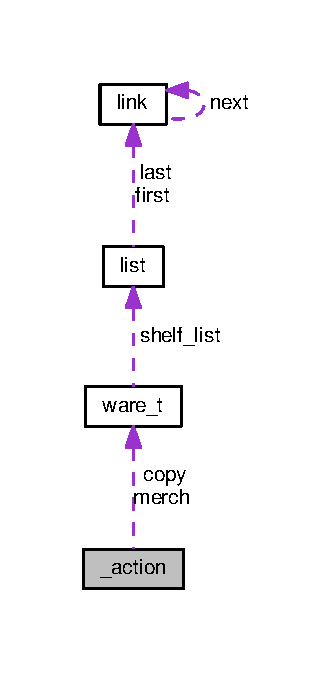
\includegraphics[width=160pt]{struct__action__coll__graph}
\end{center}
\end{figure}
\subsection*{Public Attributes}
\begin{DoxyCompactItemize}
\item 
int {\bfseries type}\hypertarget{struct__action_a8ba687cc0799b7fdda3f17732064f01b}{}\label{struct__action_a8ba687cc0799b7fdda3f17732064f01b}

\item 
\hyperlink{structware__t}{ware} $\ast$ {\bfseries merch}\hypertarget{struct__action_a7f870b5117a99cd4f9673453dc15fbc2}{}\label{struct__action_a7f870b5117a99cd4f9673453dc15fbc2}

\item 
\hyperlink{structware__t}{ware} {\bfseries copy}\hypertarget{struct__action_a015d51197547226b2711e0d3ba14ad2b}{}\label{struct__action_a015d51197547226b2711e0d3ba14ad2b}

\end{DoxyCompactItemize}


The documentation for this struct was generated from the following file\+:\begin{DoxyCompactItemize}
\item 
main.\+c\end{DoxyCompactItemize}

\hypertarget{struct__shelf}{}\section{\+\_\+shelf Struct Reference}
\label{struct__shelf}\index{\+\_\+shelf@{\+\_\+shelf}}
\subsection*{Public Attributes}
\begin{DoxyCompactItemize}
\item 
char $\ast$ {\bfseries shelf\+\_\+address}\hypertarget{struct__shelf_a8791d1ccd2e7d9d21bc27383f4a6bae5}{}\label{struct__shelf_a8791d1ccd2e7d9d21bc27383f4a6bae5}

\item 
int {\bfseries quantity}\hypertarget{struct__shelf_a06d08b16085256ece71bc65ebc1d4867}{}\label{struct__shelf_a06d08b16085256ece71bc65ebc1d4867}

\end{DoxyCompactItemize}


The documentation for this struct was generated from the following file\+:\begin{DoxyCompactItemize}
\item 
shelf.\+c\end{DoxyCompactItemize}

\hypertarget{unionanswer}{}\section{answer Union Reference}
\label{unionanswer}\index{answer@{answer}}
\subsection*{Public Attributes}
\begin{DoxyCompactItemize}
\item 
int {\bfseries i}\hypertarget{unionanswer_ab9581dbea3c0dbaf8a719b5b84323a34}{}\label{unionanswer_ab9581dbea3c0dbaf8a719b5b84323a34}

\item 
float {\bfseries f}\hypertarget{unionanswer_aa8b5513fa98d8e91d3799947ded1bf21}{}\label{unionanswer_aa8b5513fa98d8e91d3799947ded1bf21}

\item 
char $\ast$ {\bfseries s}\hypertarget{unionanswer_aabec9430aa5dd05dc5ca50a48cfebb56}{}\label{unionanswer_aabec9430aa5dd05dc5ca50a48cfebb56}

\end{DoxyCompactItemize}


The documentation for this union was generated from the following file\+:\begin{DoxyCompactItemize}
\item 
utilise.\+c\end{DoxyCompactItemize}

\hypertarget{structBrief}{}\section{Brief Struct Reference}
\label{structBrief}\index{Brief@{Brief}}


\subsection{Detailed Description}
\textbackslash{} brief elemnt is member of structure node \textbackslash{} brief left is member of structure node \textbackslash{} brief right is member of structure node struct for node holds void pointer as element and left and right subnode, which provide a bulding block for larger database creation

\textbackslash{} brief root is member of structure tree struct for node holds void pointer as element and left and right subnode, which provide a bulding block for larger database creation 

The documentation for this struct was generated from the following file\+:\begin{DoxyCompactItemize}
\item 
tree.\+c\end{DoxyCompactItemize}

\hypertarget{structlink}{}\section{link Struct Reference}
\label{structlink}\index{link@{link}}


Collaboration diagram for link\+:
\nopagebreak
\begin{figure}[H]
\begin{center}
\leavevmode
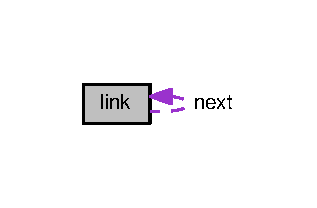
\includegraphics[width=152pt]{structlink__coll__graph}
\end{center}
\end{figure}
\subsection*{Public Attributes}
\begin{DoxyCompactItemize}
\item 
void $\ast$ {\bfseries shelf\+Name}\hypertarget{structlink_a9b099dd6c6a8b1268a687b35f826909d}{}\label{structlink_a9b099dd6c6a8b1268a687b35f826909d}

\item 
struct \hyperlink{structlink}{link} $\ast$ {\bfseries next}\hypertarget{structlink_a7d3b312c211d4e29a3a7df6c5219b923}{}\label{structlink_a7d3b312c211d4e29a3a7df6c5219b923}

\end{DoxyCompactItemize}


The documentation for this struct was generated from the following file\+:\begin{DoxyCompactItemize}
\item 
list.\+c\end{DoxyCompactItemize}

\hypertarget{structlist}{}\section{list Struct Reference}
\label{structlist}\index{list@{list}}


Collaboration diagram for list\+:
\nopagebreak
\begin{figure}[H]
\begin{center}
\leavevmode
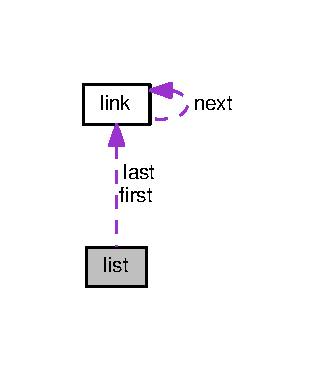
\includegraphics[width=152pt]{structlist__coll__graph}
\end{center}
\end{figure}
\subsection*{Public Attributes}
\begin{DoxyCompactItemize}
\item 
struct \hyperlink{structlink}{link} $\ast$ {\bfseries first}\hypertarget{structlist_a150377eb7a795b73db20b6c9aa6142a1}{}\label{structlist_a150377eb7a795b73db20b6c9aa6142a1}

\item 
struct \hyperlink{structlink}{link} $\ast$ {\bfseries last}\hypertarget{structlist_a8a76dcf4fdaef331b9e58f1088960163}{}\label{structlist_a8a76dcf4fdaef331b9e58f1088960163}

\end{DoxyCompactItemize}


The documentation for this struct was generated from the following file\+:\begin{DoxyCompactItemize}
\item 
list.\+c\end{DoxyCompactItemize}

\hypertarget{structnode}{}\section{node Struct Reference}
\label{structnode}\index{node@{node}}


Collaboration diagram for node\+:
\nopagebreak
\begin{figure}[H]
\begin{center}
\leavevmode
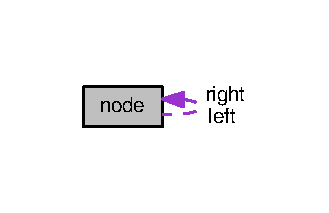
\includegraphics[width=158pt]{structnode__coll__graph}
\end{center}
\end{figure}
\subsection*{Public Attributes}
\begin{DoxyCompactItemize}
\item 
void $\ast$ \hyperlink{structnode_a3cbe5eca4f32f35778d638fb8ba4a129}{element}
\item 
struct \hyperlink{structnode}{node} $\ast$ {\bfseries left}\hypertarget{structnode_a3ce38490a651bfda86d88ff955e96abc}{}\label{structnode_a3ce38490a651bfda86d88ff955e96abc}

\item 
struct \hyperlink{structnode}{node} $\ast$ {\bfseries right}\hypertarget{structnode_a875f75abfe22103500535b179828e4e3}{}\label{structnode_a875f75abfe22103500535b179828e4e3}

\end{DoxyCompactItemize}


\subsection{Member Data Documentation}
\index{node@{node}!element@{element}}
\index{element@{element}!node@{node}}
\subsubsection[{\texorpdfstring{element}{element}}]{\setlength{\rightskip}{0pt plus 5cm}void$\ast$ node\+::element}\hypertarget{structnode_a3cbe5eca4f32f35778d638fb8ba4a129}{}\label{structnode_a3cbe5eca4f32f35778d638fb8ba4a129}
void pointer to 

The documentation for this struct was generated from the following file\+:\begin{DoxyCompactItemize}
\item 
tree.\+c\end{DoxyCompactItemize}

\hypertarget{structtree}{}\section{tree Struct Reference}
\label{structtree}\index{tree@{tree}}


Collaboration diagram for tree\+:
\nopagebreak
\begin{figure}[H]
\begin{center}
\leavevmode
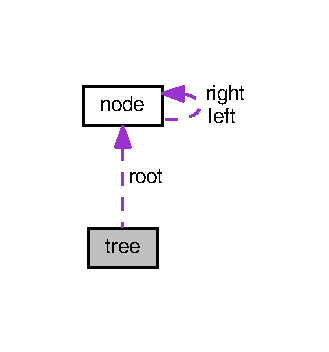
\includegraphics[width=158pt]{structtree__coll__graph}
\end{center}
\end{figure}
\subsection*{Public Attributes}
\begin{DoxyCompactItemize}
\item 
struct \hyperlink{structnode}{node} $\ast$ {\bfseries root}\hypertarget{structtree_a0739285fd0d3128fb4997c42cbfa6d0e}{}\label{structtree_a0739285fd0d3128fb4997c42cbfa6d0e}

\end{DoxyCompactItemize}


The documentation for this struct was generated from the following file\+:\begin{DoxyCompactItemize}
\item 
tree.\+c\end{DoxyCompactItemize}

\hypertarget{structware__t}{}\section{ware\+\_\+t Struct Reference}
\label{structware__t}\index{ware\+\_\+t@{ware\+\_\+t}}


Collaboration diagram for ware\+\_\+t\+:
\nopagebreak
\begin{figure}[H]
\begin{center}
\leavevmode
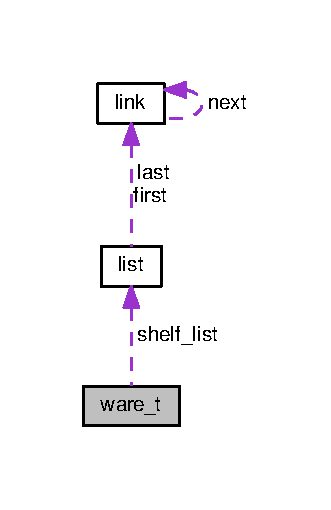
\includegraphics[width=159pt]{structware__t__coll__graph}
\end{center}
\end{figure}
\subsection*{Public Attributes}
\begin{DoxyCompactItemize}
\item 
char $\ast$ {\bfseries name}\hypertarget{structware__t_ae3630d1ec6e5c59be2b14f07a0deb8ca}{}\label{structware__t_ae3630d1ec6e5c59be2b14f07a0deb8ca}

\item 
char $\ast$ {\bfseries description}\hypertarget{structware__t_a14244f153d4dc3ea1700ea75fb716626}{}\label{structware__t_a14244f153d4dc3ea1700ea75fb716626}

\item 
int {\bfseries price}\hypertarget{structware__t_a6a2d989398ac414ccd19c6eaf9462e7c}{}\label{structware__t_a6a2d989398ac414ccd19c6eaf9462e7c}

\item 
\hyperlink{list_8h_a15376354e4e8b4f1732e9df17f30786c}{list\+\_\+t} $\ast$ {\bfseries shelf\+\_\+list}\hypertarget{structware__t_a11fe121f07b461a1d3eb25e384b12bab}{}\label{structware__t_a11fe121f07b461a1d3eb25e384b12bab}

\end{DoxyCompactItemize}


The documentation for this struct was generated from the following file\+:\begin{DoxyCompactItemize}
\item 
ware.\+h\end{DoxyCompactItemize}

\chapter{File Documentation}
\hypertarget{list_8h}{}\section{list.\+h File Reference}
\label{list_8h}\index{list.\+h@{list.\+h}}
{\ttfamily \#include $<$stdbool.\+h$>$}\\*
{\ttfamily \#include \char`\"{}shelf.\+h\char`\"{}}\\*
Include dependency graph for list.\+h\+:
\nopagebreak
\begin{figure}[H]
\begin{center}
\leavevmode
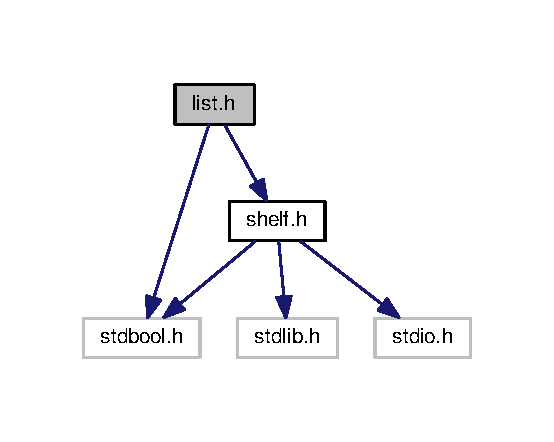
\includegraphics[width=266pt]{list_8h__incl}
\end{center}
\end{figure}
This graph shows which files directly or indirectly include this file\+:
\nopagebreak
\begin{figure}[H]
\begin{center}
\leavevmode
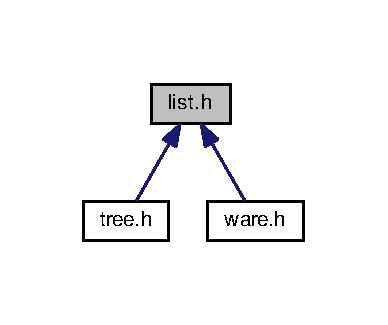
\includegraphics[width=186pt]{list_8h__dep__incl}
\end{center}
\end{figure}
\subsection*{Typedefs}
\begin{DoxyCompactItemize}
\item 
typedef struct \hyperlink{structlist}{list} \hyperlink{list_8h_a15376354e4e8b4f1732e9df17f30786c}{list\+\_\+t}
\begin{DoxyCompactList}\small\item\em Define struct list in your .c file not here! (why?) \end{DoxyCompactList}\end{DoxyCompactItemize}
\subsection*{Functions}
\begin{DoxyCompactItemize}
\item 
\hyperlink{list_8h_a15376354e4e8b4f1732e9df17f30786c}{list\+\_\+t} $\ast$ \hyperlink{list_8h_a9dd3eafdb56dcc64689f78fb4acdff3f}{list\+\_\+new} ()
\item 
bool \hyperlink{list_8h_a787a27edbde0d113b275c551ced4615d}{list\+\_\+append} (\hyperlink{list_8h_a15376354e4e8b4f1732e9df17f30786c}{list\+\_\+t} $\ast$\hyperlink{structlist}{list}, void $\ast$address)
\item 
bool \hyperlink{list_8h_af55b49002b1eac150e784108f012884d}{list\+\_\+prepend} (\hyperlink{list_8h_a15376354e4e8b4f1732e9df17f30786c}{list\+\_\+t} $\ast$\hyperlink{structlist}{list}, void $\ast$address)
\item 
bool \hyperlink{list_8h_a671345471302b32ba2f6e12584ccdcc9}{list\+\_\+insert} (\hyperlink{list_8h_a15376354e4e8b4f1732e9df17f30786c}{list\+\_\+t} $\ast$\hyperlink{structlist}{list}, int index, void $\ast$address)
\item 
bool \hyperlink{list_8h_afce3bbc1de4b555ecca0e087fef92c34}{list\+\_\+remove} (\hyperlink{list_8h_a15376354e4e8b4f1732e9df17f30786c}{list\+\_\+t} $\ast$\hyperlink{structlist}{list}, int index, void $\ast$address)
\item 
void $\ast$ \hyperlink{list_8h_a0278130929496f5e6996e52eff60f342}{list\+\_\+get} (\hyperlink{list_8h_a15376354e4e8b4f1732e9df17f30786c}{list\+\_\+t} $\ast$\hyperlink{structlist}{list}, int index)
\item 
void $\ast$ \hyperlink{list_8h_a17db498966456a086b9a49ba695a3ee0}{list\+\_\+first} (\hyperlink{list_8h_a15376354e4e8b4f1732e9df17f30786c}{list\+\_\+t} $\ast$\hyperlink{structlist}{list})\hypertarget{list_8h_a17db498966456a086b9a49ba695a3ee0}{}\label{list_8h_a17db498966456a086b9a49ba695a3ee0}

\begin{DoxyCompactList}\small\item\em A convenience for list\+\_\+get(list, 0) \end{DoxyCompactList}\item 
void $\ast$ \hyperlink{list_8h_ab7f6d8c5a8786a63042d185816b0e0a7}{list\+\_\+last} (\hyperlink{list_8h_a15376354e4e8b4f1732e9df17f30786c}{list\+\_\+t} $\ast$\hyperlink{structlist}{list})\hypertarget{list_8h_ab7f6d8c5a8786a63042d185816b0e0a7}{}\label{list_8h_ab7f6d8c5a8786a63042d185816b0e0a7}

\begin{DoxyCompactList}\small\item\em A convenience for list\+\_\+get(list, -\/1) \end{DoxyCompactList}\item 
int \hyperlink{list_8h_a95d76edca6b694b79ec54acd31fe0b82}{list\+\_\+length} (\hyperlink{list_8h_a15376354e4e8b4f1732e9df17f30786c}{list\+\_\+t} $\ast$\hyperlink{structlist}{list})
\item 
bool {\bfseries isexist} (\hyperlink{list_8h_a15376354e4e8b4f1732e9df17f30786c}{list\+\_\+t} $\ast$head, void $\ast$address)\hypertarget{list_8h_aa0217319f306eccce6dc82f70dd70a49}{}\label{list_8h_aa0217319f306eccce6dc82f70dd70a49}

\item 
void $\ast$ {\bfseries return\+\_\+shelf} (\hyperlink{list_8h_a15376354e4e8b4f1732e9df17f30786c}{list\+\_\+t} $\ast$head)\hypertarget{list_8h_abfa970c96df9ea46198b75ef9988353f}{}\label{list_8h_abfa970c96df9ea46198b75ef9988353f}

\item 
void {\bfseries print\+\_\+link\+\_\+list} (\hyperlink{list_8h_a15376354e4e8b4f1732e9df17f30786c}{list\+\_\+t} $\ast$head)\hypertarget{list_8h_ae01d4f5455db767c41da137eb1b9b373}{}\label{list_8h_ae01d4f5455db767c41da137eb1b9b373}

\item 
void $\ast$ {\bfseries list\+Getshelf} (\hyperlink{list_8h_a15376354e4e8b4f1732e9df17f30786c}{list\+\_\+t} $\ast$head, int index)\hypertarget{list_8h_a23779d12ed4bc50fb57634a578979340}{}\label{list_8h_a23779d12ed4bc50fb57634a578979340}

\end{DoxyCompactItemize}


\subsection{Detailed Description}
\begin{DoxyAuthor}{Author}
Tobias Wrigstad 
\end{DoxyAuthor}
\begin{DoxyVersion}{Version}
1.\+0 
\end{DoxyVersion}
\begin{DoxyDate}{Date}
2015-\/08-\/28 
\end{DoxyDate}
\begin{DoxyRefDesc}{Bug}
\item[\hyperlink{bug__bug000001}{Bug}]None known. But this code is untested so there are likely bigs in it. \end{DoxyRefDesc}


\subsection{Typedef Documentation}
\index{list.\+h@{list.\+h}!list\+\_\+t@{list\+\_\+t}}
\index{list\+\_\+t@{list\+\_\+t}!list.\+h@{list.\+h}}
\subsubsection[{\texorpdfstring{list\+\_\+t}{list_t}}]{\setlength{\rightskip}{0pt plus 5cm}typedef struct {\bf list} {\bf list\+\_\+t}}\hypertarget{list_8h_a15376354e4e8b4f1732e9df17f30786c}{}\label{list_8h_a15376354e4e8b4f1732e9df17f30786c}


Define struct list in your .c file not here! (why?) 

!! O\+BS -- du kommer att behöva ändra lite i denna fil. !! Detta är en lista som endast hanterar heltal. Men det !! kommer inte att räcka för oss här eftersom vi skall ha !! andra data (vilka??) i vår (enda) lista. 

\subsection{Function Documentation}
\index{list.\+h@{list.\+h}!list\+\_\+append@{list\+\_\+append}}
\index{list\+\_\+append@{list\+\_\+append}!list.\+h@{list.\+h}}
\subsubsection[{\texorpdfstring{list\+\_\+append(list\+\_\+t $\ast$list, void $\ast$address)}{list_append(list_t *list, void *address)}}]{\setlength{\rightskip}{0pt plus 5cm}bool list\+\_\+append (
\begin{DoxyParamCaption}
\item[{{\bf list\+\_\+t} $\ast$}]{list, }
\item[{void $\ast$}]{address}
\end{DoxyParamCaption}
)}\hypertarget{list_8h_a787a27edbde0d113b275c551ced4615d}{}\label{list_8h_a787a27edbde0d113b275c551ced4615d}
Inserts a new element at the end of the list


\begin{DoxyParams}{Parameters}
{\em list} & pointer to the list \\
\hline
{\em elem} & the integer to be appended \\
\hline
\end{DoxyParams}
\index{list.\+h@{list.\+h}!list\+\_\+get@{list\+\_\+get}}
\index{list\+\_\+get@{list\+\_\+get}!list.\+h@{list.\+h}}
\subsubsection[{\texorpdfstring{list\+\_\+get(list\+\_\+t $\ast$list, int index)}{list_get(list_t *list, int index)}}]{\setlength{\rightskip}{0pt plus 5cm}void$\ast$ list\+\_\+get (
\begin{DoxyParamCaption}
\item[{{\bf list\+\_\+t} $\ast$}]{list, }
\item[{int}]{index}
\end{DoxyParamCaption}
)}\hypertarget{list_8h_a0278130929496f5e6996e52eff60f342}{}\label{list_8h_a0278130929496f5e6996e52eff60f342}
Returns the element at a given index 
\begin{DoxyParams}{Parameters}
{\em list} & pointer to the list \\
\hline
{\em index} & the index to be returns \\
\hline
\end{DoxyParams}
\begin{DoxyReturn}{Returns}
a pointer to the element at index index 
\end{DoxyReturn}
\index{list.\+h@{list.\+h}!list\+\_\+insert@{list\+\_\+insert}}
\index{list\+\_\+insert@{list\+\_\+insert}!list.\+h@{list.\+h}}
\subsubsection[{\texorpdfstring{list\+\_\+insert(list\+\_\+t $\ast$list, int index, void $\ast$address)}{list_insert(list_t *list, int index, void *address)}}]{\setlength{\rightskip}{0pt plus 5cm}bool list\+\_\+insert (
\begin{DoxyParamCaption}
\item[{{\bf list\+\_\+t} $\ast$}]{list, }
\item[{int}]{index, }
\item[{void $\ast$}]{address}
\end{DoxyParamCaption}
)}\hypertarget{list_8h_a671345471302b32ba2f6e12584ccdcc9}{}\label{list_8h_a671345471302b32ba2f6e12584ccdcc9}
Inserts a new element at a given index.

Valid indexes are \mbox{[}0..size\mbox{]}.

Example\+:

list\+\_\+t $\ast$l = \hyperlink{list_8h_a9dd3eafdb56dcc64689f78fb4acdff3f}{list\+\_\+new()}; // l == \mbox{[}\mbox{]} list\+\_\+insert(l, 0, 42); // l == \mbox{[}42\mbox{]} list\+\_\+insert(l, 0, 43); // l == \mbox{[}43, 42\mbox{]} list\+\_\+insert(l, 1, 44); // l == \mbox{[}43, 44, 42\mbox{]} list\+\_\+insert(l, 5, 45); // l == \mbox{[}43, 44, 42\mbox{]}

The last case fails (and returns false) because size is 3, meaning 5 is not a valid index.

Note that insert at index 0 is the same as prepend and insert index size is the same as append.

Negative indexes should be supported\+:

list\+\_\+insert(l, -\/1, 45); // l == \mbox{[}43, 44, 42, 45\mbox{]}

A positive index can be calculated from a negative like this\+: pos\+\_\+i = size + 1 + neg\+\_\+i.


\begin{DoxyParams}{Parameters}
{\em list} & pointer to the list \\
\hline
{\em index} & the index for elem to be inserted at \\
\hline
{\em elem} & the integer to be prepended \\
\hline
\end{DoxyParams}
\begin{DoxyReturn}{Returns}
true if succeeded, else false 
\end{DoxyReturn}
\index{list.\+h@{list.\+h}!list\+\_\+length@{list\+\_\+length}}
\index{list\+\_\+length@{list\+\_\+length}!list.\+h@{list.\+h}}
\subsubsection[{\texorpdfstring{list\+\_\+length(list\+\_\+t $\ast$list)}{list_length(list_t *list)}}]{\setlength{\rightskip}{0pt plus 5cm}int list\+\_\+length (
\begin{DoxyParamCaption}
\item[{{\bf list\+\_\+t} $\ast$}]{list}
\end{DoxyParamCaption}
)}\hypertarget{list_8h_a95d76edca6b694b79ec54acd31fe0b82}{}\label{list_8h_a95d76edca6b694b79ec54acd31fe0b82}
Returns the length of the list. It is undefined whether the length is calculated in O(n) time or whether there is a size counter in the list object that is manipulated by insert, remove, etc. 
\begin{DoxyParams}{Parameters}
{\em list} & the list \\
\hline
\end{DoxyParams}
\begin{DoxyReturn}{Returns}
the length of list 
\end{DoxyReturn}
\index{list.\+h@{list.\+h}!list\+\_\+new@{list\+\_\+new}}
\index{list\+\_\+new@{list\+\_\+new}!list.\+h@{list.\+h}}
\subsubsection[{\texorpdfstring{list\+\_\+new()}{list_new()}}]{\setlength{\rightskip}{0pt plus 5cm}{\bf list\+\_\+t}$\ast$ list\+\_\+new (
\begin{DoxyParamCaption}
{}
\end{DoxyParamCaption}
)}\hypertarget{list_8h_a9dd3eafdb56dcc64689f78fb4acdff3f}{}\label{list_8h_a9dd3eafdb56dcc64689f78fb4acdff3f}
Creates a new list

\begin{DoxyReturn}{Returns}
\+: empty list 
\end{DoxyReturn}
\index{list.\+h@{list.\+h}!list\+\_\+prepend@{list\+\_\+prepend}}
\index{list\+\_\+prepend@{list\+\_\+prepend}!list.\+h@{list.\+h}}
\subsubsection[{\texorpdfstring{list\+\_\+prepend(list\+\_\+t $\ast$list, void $\ast$address)}{list_prepend(list_t *list, void *address)}}]{\setlength{\rightskip}{0pt plus 5cm}bool list\+\_\+prepend (
\begin{DoxyParamCaption}
\item[{{\bf list\+\_\+t} $\ast$}]{list, }
\item[{void $\ast$}]{address}
\end{DoxyParamCaption}
)}\hypertarget{list_8h_af55b49002b1eac150e784108f012884d}{}\label{list_8h_af55b49002b1eac150e784108f012884d}
Inserts a new element at the end of the list


\begin{DoxyParams}{Parameters}
{\em list} & pointer to the list \\
\hline
{\em elem} & the integer to be prepended \\
\hline
\end{DoxyParams}
\index{list.\+h@{list.\+h}!list\+\_\+remove@{list\+\_\+remove}}
\index{list\+\_\+remove@{list\+\_\+remove}!list.\+h@{list.\+h}}
\subsubsection[{\texorpdfstring{list\+\_\+remove(list\+\_\+t $\ast$list, int index, void $\ast$address)}{list_remove(list_t *list, int index, void *address)}}]{\setlength{\rightskip}{0pt plus 5cm}bool list\+\_\+remove (
\begin{DoxyParamCaption}
\item[{{\bf list\+\_\+t} $\ast$}]{list, }
\item[{int}]{index, }
\item[{void $\ast$}]{address}
\end{DoxyParamCaption}
)}\hypertarget{list_8h_afce3bbc1de4b555ecca0e087fef92c34}{}\label{list_8h_afce3bbc1de4b555ecca0e087fef92c34}
Removes an element from a list.

Example\+: (assume l == \mbox{[}43, 44, 42, 45\mbox{]})

int elem; list\+\_\+remove(l, 1, \&elem); // l = \mbox{[}43, 42, 45\mbox{]}, elem == 44 list\+\_\+remove(l, -\/1, \&elem); // l = \mbox{[}43, 42\mbox{]}, elem == 45


\begin{DoxyParams}{Parameters}
{\em list} & pointer to the list \\
\hline
{\em index} & the index to be removed \\
\hline
{\em elem} & a pointer to where the element can be stored \\
\hline
\end{DoxyParams}
\begin{DoxyReturn}{Returns}
true if succeeded, else 
\end{DoxyReturn}

%--- End generated contents ---

% Index
\backmatter
\newpage
\phantomsection
\clearemptydoublepage
\addcontentsline{toc}{chapter}{Index}
\printindex

\end{document}
